\documentclass{standalone}
\usepackage{tikz}
\usepackage{ctex,siunitx,upgreek}
\setCJKmainfont{Noto Serif CJK SC}
\usepackage{tkz-euclide}
\usepackage{amsmath,amsfonts,amssymb}
\usetikzlibrary{patterns, calc,3d}
\usetikzlibrary {decorations.pathmorphing,decorations.pathreplacing,decorations.shapes}
\tikzset{label style/.append style={font=\small}}
\begin{document}
\small
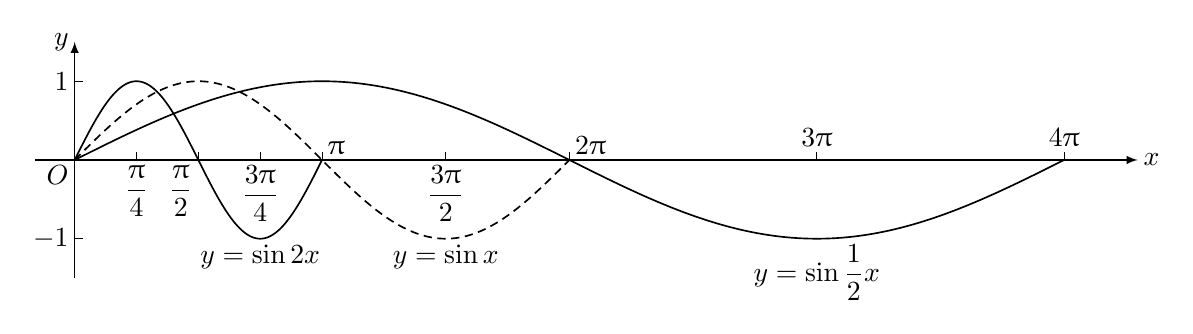
\begin{tikzpicture}[>=latex,scale=1.0,inner sep=2pt]
  \draw[->](-0.5,0)--(13.5,0)node[right]{$x$};
  \draw[->](0,-1.5)--(0,1.5)node[left]{$y$};
  \node at (0,0)[below left]{$O$};
  \draw[semithick,samples=200,domain=0:4*pi]plot(\x,{sin(0.5*\x r)});
  \draw[semithick,densely dashed,samples=200,domain=0:2*pi]plot(\x,{sin(\x r)});
  \draw[semithick,samples=200,domain=0:pi]plot(\x,{sin(2*\x r)});
  \foreach \x in {-1,1} {\draw(0,\x)node[left]{$\x$}--++(0.1,0);}
  \draw[very thin](0.25*pi,0)node[below]{$\dfrac\uppi4$}--++(0,0.1);
  \draw[very thin](0.5*pi,0)node[below left]{$\dfrac\uppi2$}--++(0,0.1);
  \draw[very thin](0.75*pi,0)node[below]{$\dfrac{3\uppi}{4}$}--++(0,0.1);
  \draw[very thin](pi,0)node[above right]{$\uppi$}--++(0,0.1);
  \draw[very thin](2*pi,0)node[above right]{$2\uppi$}--++(0,0.1);
  \draw[very thin](3*pi,0)--++(0,0.1)node[above]{$3\uppi$};
  \draw[very thin](4*pi,0)--++(0,0.1)node[above]{$4\uppi$};
  \draw[very thin](1.5*pi,0)node[below]{$\dfrac{3\uppi}{2}$}--++(0,0.1);
  \node at (0.75*pi,-1)[below]{$y=\sin2x$};
  \node at (1.5*pi,-1)[below]{$y=\sin x$};
  \node at (3*pi,-1)[below]{$y=\sin\dfrac12x$};
\end{tikzpicture}
\end{document}